\documentclass[11pt]{article}

\usepackage[a4paper]{geometry}
\geometry{left=2.0cm,right=2.0cm,top=2.5cm,bottom=2.5cm}

\usepackage{ctex} % 支持中文的LaTeX宏包
\usepackage{amsmath,amsfonts,graphicx,subfigure,amssymb,bm,amsthm,mathrsfs,mathtools,breqn} % 数学公式和符号的宏包集合
\usepackage{algorithm,algorithmicx} % 算法和伪代码的宏包
\usepackage[noend]{algpseudocode} % 算法和伪代码的宏包
\usepackage{fancyhdr} % 自定义页眉页脚的宏包
\usepackage[framemethod=TikZ]{mdframed} % 创建带边框的框架的宏包
\usepackage{fontspec} % 字体设置的宏包
\usepackage{adjustbox} % 调整盒子大小的宏包
\usepackage{fontsize} % 设置字体大小的宏包
\usepackage{tikz,xcolor} % 绘制图形和使用颜色的宏包
\usepackage{multicol} % 多栏排版的宏包
\usepackage{multirow} % 表格中合并单元格的宏包
\usepackage{pdfpages} % 插入PDF文件的宏包
\RequirePackage{listings} % 在文档中插入源代码的宏包
\RequirePackage{xcolor} % 定义和使用颜色的宏包
\usepackage{wrapfig} % 文字绕排图片的宏包
\usepackage{bigstrut,multirow,rotating} % 支持在表格中使用特殊命令的宏包
\usepackage{booktabs} % 创建美观的表格的宏包
\usepackage{circuitikz} % 绘制电路图的宏包
\usepackage{caption}
\usepackage{amsmath} % 必需
\captionsetup{font=normalsize,skip=2pt}

\definecolor{dkgreen}{rgb}{0,0.6,0}
\definecolor{gray}{rgb}{0.5,0.5,0.5}
\definecolor{mauve}{rgb}{0.58,0,0.82}
\lstset{
  frame=tb,
  aboveskip=3mm,
  belowskip=3mm,
  showstringspaces=false,
  columns=flexible,
  framerule=1pt,
  rulecolor=\color{gray!35},
  backgroundcolor=\color{gray!5},
  basicstyle={\small\ttfamily},
  numbers=none,
  numberstyle=\tiny\color{gray},
  keywordstyle=\color{blue},
  commentstyle=\color{dkgreen},
  stringstyle=\color{mauve},
  breaklines=true,
  breakatwhitespace=true,
  tabsize=3,
}

% 轻松引用, 可以用\cref{}指令直接引用, 自动加前缀. 
% 例: 图片label为fig:1
% \cref{fig:1} => Figure.1
% \ref{fig:1}  => 1
\usepackage[capitalize]{cleveref}
% \crefname{section}{Sec.}{Secs.}
\Crefname{section}{Section}{Sections}
\Crefname{table}{Table}{Tables}
\crefname{table}{Table.}{Tabs.}

\setmainfont{Palatino_Linotype}[
  Path = ../Fonts/,
  Extension = .ttf
]
\setCJKmainfont{SimHei}[
  Path = ../Fonts/,
  Extension = .ttf
]
\punctstyle{kaiming}
% 偏好的几个字体, 可以根据需要自行加入字体ttf文件并调用

\renewcommand{\emph}[1]{\begin{kaishu}#1\end{kaishu}}

%改这里可以修改实验报告表头的信息
\newcommand{\studentNum}{00000000}
\newcommand{\name}{我是谁}
\newcommand{\exDate}{2025.05.06}
\newcommand{\weekDay}{二}
\newcommand{\ap}{下午}
%%%%%%%%%%%%%%%%%%%%%%%%%%%

\begin{document}

%若需在页眉部分加入内容, 可以在这里输入
% \pagestyle{fancy}
% \lhead{\kaishu 测试}
% \chead{}
% \rhead{}

\begin{center}
    \LARGE \bf 《\, 基\, 础\, 物\, 理\, 实\, 验\, 》\, 实\, 验\, 报\, 告
\end{center}

\begin{center}
    \emph{学号}\underline{\makebox[6em][c]{\studentNum}}
    \emph{姓名}\underline{\makebox[6em][c]{\name}} 
    \emph{实验日期} \underline{\makebox[8em][c]{\exDate}}
    \emph{星期} \underline{\makebox[2em][c]{\weekDay}}\;\underline{\makebox[3em][c]{\ap}}
    {\noindent}
    \rule[8pt]{17cm}{0.2em}
\end{center}

\begin{center}
    \Large \bf 空气比热容比的测定
\end{center}

\section*{一、实验目的}

\begin{enumerate}
    \item 用绝热膨胀法测定空气的比热容比。
    \item 观测热力学过程中状态变化及基本物理规律。
\end{enumerate}

\section*{二、实验仪器}

空气比热容测定仪(含AD590温度传感器和扩散硅压力传感器)、温度计(测室温)、气压计(测环境气压)。

\section*{三、实验原理}

\begin{wrapfigure}{r}{3cm}
    \centering
    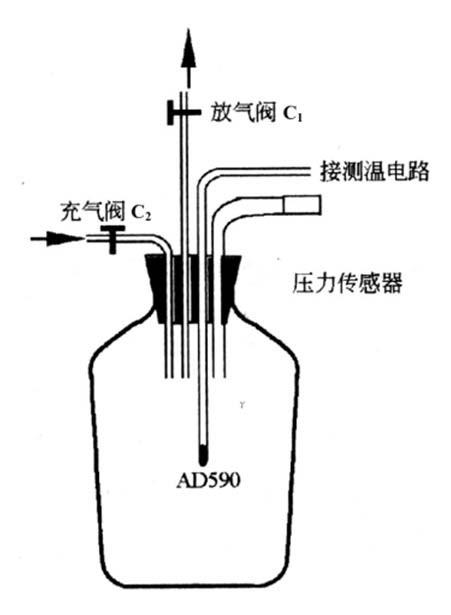
\includegraphics[width=3cm]{Figs/实验装置图.jpg}
    \caption{\small 实验装置图}
\end{wrapfigure}

理想气体的压强$P$、体积$V$和温度$T$在准静态绝热过程中,遵守绝热过程方程:$PV^\gamma$等于恒量,其中$\gamma$是气体的定压比热容$C_P$和定容比热容$C_V$之比,通常称$\gamma=\dfrac{C_P}{C_V}$为该气体的比热容比(亦称绝热指数)。如图1所示,我们以贮气瓶内空气(近似为理想气体)作为研究的热学系统,试进行如下实验过程。\\
(1) 首先打开放气阀$C_1$,贮气瓶与大气相通,再关闭$C_1$,瓶内充满与周围空气同温(设为$T_0$)同压(设为$P_0$)的气体。\\
(2) 打开充气阀$C_2$用充气球向瓶内打气,充入一定量的气体,然后关闭充气阀$C_2$。此时瓶内空气被压缩,压强增大,温度升高。等待内部气体温度稳定,即达到与周围温度平衡,此时的研究的气体处于状态\uppercase\expandafter{\romannumeral1}$(P_1,V_1,T_0)$。虽然瓶内气体的体积为贮气瓶容积$V_0$,而仅有$V_1$部分($V_1<V_0$)是实验研究的对象,如图2。\\
(3) 迅速打开放气阀$C_1$,使瓶内气体与大气相通,当瓶内压强降至$P_0$时,立刻关闭放气阀$C_1$将有体积为$\Delta V$的气体喷泻出贮气瓶。由于放气过程较快,瓶内保留的气体来不及与外界进行热交换,可以认为是一个绝热膨胀的过程。在此过程后瓶中的气体由状态\uppercase\expandafter{\romannumeral1}$(P_1,V_1,T_0)$转变为状态\uppercase\expandafter{\romannumeral2}$(P_0,V_0,T_1)$。$V_0$为贮气瓶容积,$V_1$为保留在瓶中这部分气体在状态\uppercase\expandafter{\romannumeral1}$(P_1,T_0)$时的体积。\\
(4) 由于瓶内气体温度$T_1$低于室温$T_0$,所以瓶内气体慢慢从外界吸热,直至 达到室温$T_0$为止,此时瓶内气体压强也随之增大为$P_2$。则稳定后的气体状态为\uppercase\expandafter{\romannumeral3}$(P_2,V_0,T_0)$;从状态\uppercase\expandafter{\romannumeral2}到状态\uppercase\expandafter{\romannumeral3}的过程可以看作是一个等容吸热的过程。

\begin{figure}[H]
    \centering
    \subfigure{
        \begin{minipage}{7cm}
        \centering
        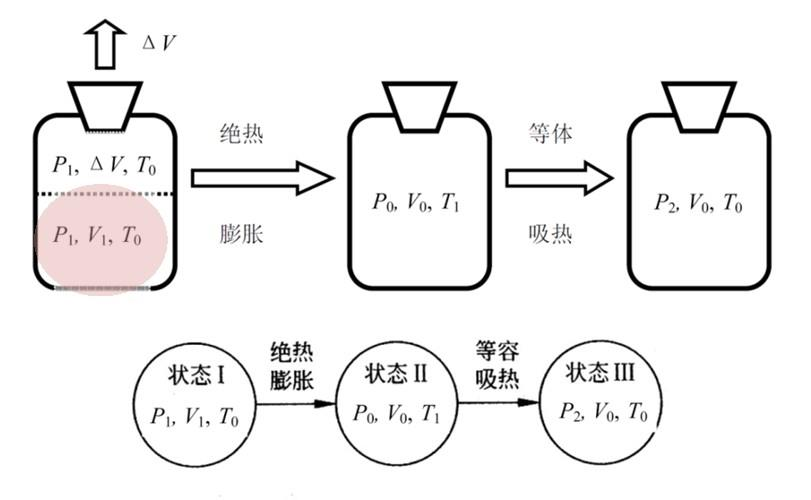
\includegraphics[scale=0.5]{Figs/气体状态变化图.jpg}
        \end{minipage}
    }
    \subfigure{
        \begin{minipage}{7cm}
        \centering
        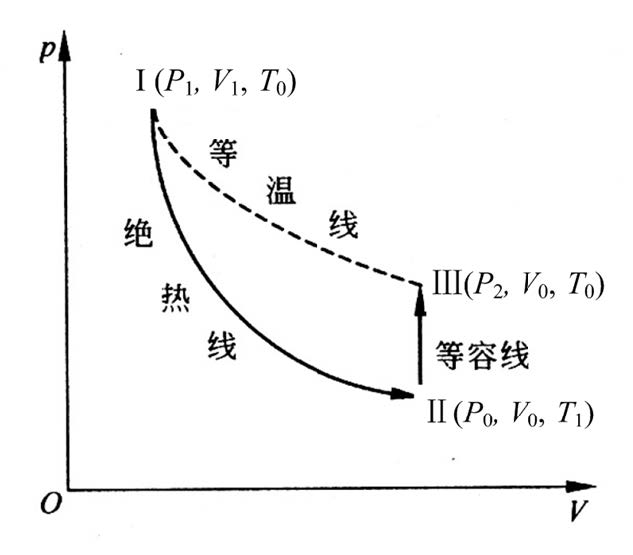
\includegraphics[scale=0.5]{Figs/PV图.jpg}
        \end{minipage}
    }
    \caption{气体状态变化及$P-V$图}
\end{figure}

由状态\uppercase\expandafter{\romannumeral1}$\rightarrow $\uppercase\expandafter{\romannumeral2}$\rightarrow $\uppercase\expandafter{\romannumeral3}的过程如图2所示。\uppercase\expandafter{\romannumeral1}$\rightarrow $\uppercase\expandafter{\romannumeral2}是绝热过程,由绝热过程方程
得:
\begin{align}
    P_1V_1^\gamma=P_0V_0^\gamma
\end{align}
状态\uppercase\expandafter{\romannumeral1}和状态\uppercase\expandafter{\romannumeral3}的温度均为$T_0$,由气体状态方程得:
\begin{align}
    P_1V_1=P_2V_0
\end{align}
合并式$(1)(2)$,消去$V_0,V_1$,得:
\begin{align}
    \gamma=\dfrac{\ln{P_1}-\ln{P_0}}{\ln{P_1}-\ln{P_2}}=\dfrac{\ln{\dfrac{P_1}{P_0}}}{\ln{\dfrac{P_1}{P_2}}}
\end{align}
由式$(3)$可以看出,只要测得$P_0,P_1,P_2$就可求得空气的绝热指数$\gamma$。本实验气瓶内的气压通过扩散硅传感器来测量,压强值通过电压值来显示,其灵敏度为$20\,mV/kPa$。当待测压强为大气压$P_0$时将电压示数调零,当压强显示读数为$P\,mV$时,实际压强为:
\begin{align}
    P(Pa)=P_0+50\times P(mV)
\end{align}
气瓶内温度通过AD590温度传感器测量,也是以电压值来显示,其灵敏度为$5mV/^{\circ}C$,最小可检测$0.02^{\circ}C$的温度变化。

\section*{四、实验内容}

\begin{enumerate}
    \item 用气压计测定大气压强$P_0(Pa)$,用温度计测环境室温$T_0(^{\circ}C)$。打开放气阀$C_1$,开启电源,让电子仪器部件预热一段时间,然后将压强指示值调到“$0$”,并记录此时温度指示值$T_0$(以$mV$为单位)。
    \item 关闭放气阀$C_1$,打开充气阀$C_2$,用充气球向瓶内打气,使压强升高到$100\,mV-120\,mV$。然后关闭充气阀$C_2$,当瓶内气体压强和温度的指示值不变时,气体处于状态\uppercase\expandafter{\romannumeral1},记下压强$P_1$和温度$T_1$(以$mV$为单位)。
    \item 迅速打开放气阀$C_1$,当放气声消失时立刻关闭放气阀$C_1$,此时瓶内空气压强降至大气压强$P_0$,气体温度降低,气体处于状态\uppercase\expandafter{\romannumeral2}。
    \item 待瓶内气体的温度上升稳定,且压强也稳定后,此时瓶内气体近处于状态\uppercase\expandafter{\romannumeral3},记录压强$P_2$和温度$T_2$。
    \item 打开放气阀$C_1$使贮气瓶与大气相通,以便于下一次测量。
    \item 重复步骤$2-4$,重复$10$次测量,比较多次测量中气体的状态变化有何异同,并计算$\overline{\gamma}$,分析误差,利用统计规律公式$\sqrt{\dfrac{\sum_{i=1}^{n}(x_i-\overline{x})^2}{n-1}}$,计算实验结果的随机涨落偏差。
    \item 放气时间过长,重复步骤$2-4$,重复$5$次测量,计算$\overline{\gamma_1}$。
    \item 放气时间不充分,重复步骤$2-4$,重复$5$次测量,计算$\overline{\gamma_2}$。
    \item 比较三种情况的测量平均值,与理论值$1.40$比较,计算与理论值对比的相对误差$E_r=\dfrac{\overline{\gamma_i}-1.40}{1.40}\times100\%$,并分析偏离原因。
\end{enumerate}

\section*{五、数据记录}

原始数据见附页。

\section*{六、数据处理}

实验开始时$P_{0_1}=99880\,Pa$,实验结束时$P_{0_2}=99850\,Pa$,计算平均值得到$P_0=\dfrac{P_{0_1}+P_{0_2}}{2}=\\\dfrac{99880\,Pa+99850\,Pa}{2}=99865\,Pa$。通过使用Origin软件对实验数据进行处理计算$P_1, P_2, \gamma$,得到:

\begin{figure}[H]
    \centering
    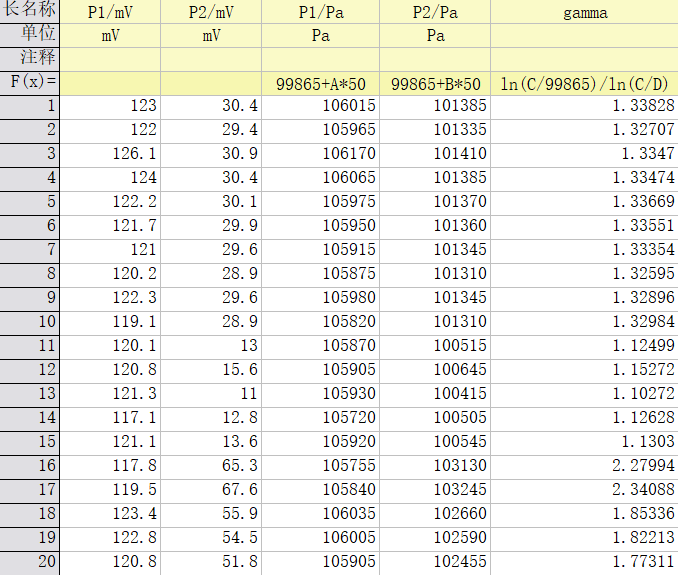
\includegraphics[width=10cm]{Figs/数据.png}
    \caption{实验数据处理结果}
\end{figure}

计算正常测量的空气比热容比的平均值
\begin{align*}
    \overline{\gamma}&=\frac{1.33828+1.32707+1.33470+1.33474+1.33669+1.33551+1.33354+1.32595+1.32896+1.32984}{10}\\
    &=1.33253\quad\text{略小于理论值}1.40
\end{align*}

计算实验结果的随机涨落偏差
\begin{align*}
    s&=\sqrt{\frac{\sum_{i=1}^n(x_i-\overline{x})^2}{n-1}}\\
    &=\sqrt{\frac{\splitfrac{\splitfrac{(1.33828-1.33253)^2+(1.32707-1.33253)^2+(1.33470-1.33253)^2}{+(1.33474-1.33253)^2+(1.33669-1.33253)^2+(1.33551-1.33253)^2}}{+(1.33354-1.33253)^2+(1.32595-1.33253)^2+(1.32896-1.33253)^2+(1.32984-1.33253)^2}}{10-1}}\\
    &=0.004254
\end{align*}

计算放气时间过长的空气比热容比的平均值
\begin{align*}
    \overline{\gamma_1}&=\frac{1.12499+1.15272+1.10272+1.12628+1.13030}{5}\\
    &=1.12741\quad\text{远小于理论值}1.40
\end{align*}

计算放气时间不充分的空气比热容比的平均值
\begin{align*}
    \overline{\gamma_2}&=\frac{2.27994+2.34088+1.85336+1.82213+1.77311}{5}\\
    &=2.01388\quad\text{远大于理论值}1.40
\end{align*}

计算与理论值对比的相对误差
\begin{align*}
    \text{正常操作:}E_r&=\frac{|\overline{\gamma}-1.40|}{1.40}\times100\%\\
    &=\frac{|1.33253-1.40|}{1.40}\times100\%=4.82\%\\
    \text{放气过久:}E_{r_1}&=\frac{|\overline{\gamma_1}-1.40|}{1.40}\times100\%\\
    &=\frac{|1.12741-1.40|}{1.40}\times100\%=19.47\%\\
    \text{放气不充分:}E_{r_2}&=\frac{|\overline{\gamma_2}-1.40|}{1.40}\times100\%\\
    &=\frac{|2.01388-1.40|}{1.40}\times100\%=43.85\%
\end{align*}

正常操作时,气体与外界存在热交换,使测量得到的$P_2$偏小,导致计算得到的$\gamma$偏小。放气时间过长,气体有充足的时间与外界热交换,导致测量得到的$P_2$偏小,计算得到的$\gamma$偏小。放气时间不充分,内外气压未达到平衡,导致测量得到的$P_2$偏大,计算得到的$\gamma$偏大。

\section*{七、误差分析}

\begin{enumerate}
    \item 温度传感器和压力传感器的灵敏度有限,可能导致测量误差;
    \item 无法精准控制放气时间,放气时间过长或过短都会影响实验结果;
    \item 装置无法完全绝热,气体在放气以及等待平衡过程中与外界有热交换,影响了实验结果;
    \item 实验室的空调影响环境温度,导致实验室温度不稳定;
    \item 实验前后的气压与温度有变化,可能导致实验结果不准确;
    \item 平衡过程时间较长,可能提前读取结果导致结果不准确;
    \item 气体不是理想气体,实际气体的行为与理想气体有所不同,可能导致实验结果偏差。
\end{enumerate}

\section*{八、思考题}

\begin{enumerate}
    \item 为什么在实验中不需要测量状态\uppercase\expandafter{\romannumeral2}的压强和温度值?请简述理由。
    答:

    状态\uppercase\expandafter{\romannumeral2}是绝热膨胀的中间态,不稳定,难以测量;并且由公式$(3)$可知,状态\uppercase\expandafter{\romannumeral2}的压强和温度在计算$\gamma$时不需要,因此不需要测量。
    \item 在放气瞬间,瓶内气体温度有无变化?试通过热力学定律分析原因。
    答:

    有变化。根据热力学第一定律$\Delta U=Q+W$,绝热膨胀过程中,内能的变化等于做功的量,在放气瞬间,气体体积膨胀,对外做功,所以内能减少,即温度降低。
\end{enumerate}

\section*{九、实验结论}

本实验采用绝热膨胀法,测定空气的比热容比。在三种情况下分别测得正常操作时的比热容比$\overline{\gamma}=1.33253$,放气时间过长时的比热容比$\overline{\gamma_1}=1.12741$,放气时间不充分时的比热容比$\overline{\gamma_2}=2.01388$。与理论值$1.40$相比,正常操作时的相对误差为$4.82\%$,放气时间过长时的相对误差为$19.47\%$,放气时间不充分时的相对误差为$43.85\%$。实验结果表明,放气时间过长或不充分偏差较大,正常操作与理论值误差较小,实验结果的随机涨落偏差为$0.004254$,测量结果合理。

\end{document}